%%%%%%%%%%%%%%%%%%%%%%%%%%%%%%%%%%%%%%%%%%%%%%%%%%%%%%%%%%%%
%%% LIVECOMS ARTICLE TEMPLATE
%%% ADAPTED FROM ELIFE ARTICLE TEMPLATE (8/10/2017)
%%%%%%%%%%%%%%%%%%%%%%%%%%%%%%%%%%%%%%%%%%%%%%%%%%%%%%%%%%%%
%%% PREAMBLE 
\documentclass[9pt]{livecoms}
% Use the 'onehalfspacing' option for 1.5 line spacing
% Use the 'doublespacing' option for 2.0 line spacing
% use the 'lineno' option for adding line numbers. 
% Please note that these options may affect formatting.

\usepackage{lipsum} % Required to insert dummy text
\usepackage[version=4]{mhchem} 
\usepackage{siunitx}
\DeclareSIUnit\Molar{M}
\newcommand{\versionnumber}{1.3}  % you should update the minor version number in preprints and major version number of submissions.
%%%%%%%%%%%%%%%%%%%%%%%%%%%%%%%%%%%%%%%%%%%%%%%%%%%%%%%%%%%%
%%% ARTICLE SETUP
%%%%%%%%%%%%%%%%%%%%%%%%%%%%%%%%%%%%%%%%%%%%%%%%%%%%%%%%%%%%
\title{This is the title : v\versionnumber}

\author[1*,\authfn{1}\authfn{3}]{Edward Maginn}
\author[2\authfn{1}\authfn{4}]{Daniel Roe}
\author[3\authfn{1}\authfn{4}]{Richard Elliott}
\author[4\authfn{1}\authfn{4}]{Richard Messerly}
\author[5\authfn{1}\authfn{4}]{Sunny Hwang}
\affil[1]{Institution 1}
\affil[2]{Institution 2}

\corr{email1@example.com}{FMS}  % Correspondence emails.  FMS and FS are the appropriate authors initials. 
\corr{email2@example.com}{FS}

\contrib[\authfn{1}]{These authors contributed equally to this work}
\contrib[\authfn{2}]{These authors also contributed to this work}

\presentadd[\authfn{3}]{Department, Institute, Country}
\presentadd[\authfn{4}]{Department, Institute, Country}

%%%%%%%%%%%%%%%%%%%%%%%%%%%%%%%%%%%%%%%%%%%%%%%%%%%%%%%%%%%%
%%% ARTICLE START
%%%%%%%%%%%%%%%%%%%%%%%%%%%%%%%%%%%%%%%%%%%%%%%%%%%%%%%%%%%%

\begin{document}

\maketitle

\begin{abstract}
Please provide an abstract of no more than 250 words. Your abstract should explain the main contributions of your article, and should not contain any material that is not included in the main text.
\end{abstract}

%Edward Maginn (ejmaginn), Richard Elliott, Sunny Hwang, Daniel Roe (GitHub: drroe), Rich Messerly (ramess101)
%List of people to contact: Peter Cummings, Richard Rowley, Joachim Gross, Raj Khare, Richard Sadus, Ioannis Economou, Jadran Vrabec, (any other Richards we can come up with)


\section{Outline}

Separate documents for:
\begin{enumerate}
	\item Equilibrium methods (self-diffusivity, viscosity) for liquids
	\item Non-equilibrium methods (self-diffusivity, viscosity) for liquids
	\item Methods for thermal conductivity
	\item Methods for ionic conductivity
\end{enumerate}

General outline of equilibrium methods of self-diffusivity and viscosity for liquids:
\begin{enumerate}
	\item Introduction
	\item Discussion of different methods within EMD (Green-Kubo, Einstein)
	\item General simulation set-up
	\item Diffusion
	\begin{enumerate}
		\item Brief discussion of why we recommend Einstein over Green-Kubo?
		\item Simulation setup that is specific to Einstein/diffusion
		\item Data analysis specific to Einstein/diffusion
		\item Common pitfalls for Einstein/diffusion
	\end{enumerate}
	\item Viscosity
	\begin{enumerate}
		\item Brief discussion of why we recommend Green-Kubo over Einstein?
		\item Simulation setup that is specific to Green-Kubo/viscosity
		\item Data analysis specific to Green-Kubo/viscosity
		\item Common pitfalls for Green-Kubo/viscosity
	\end{enumerate}
\end{enumerate}


\section{Introduction}

Transport properties describe the rates at which mass, momentum, heat or charge move through a given substance. They involve mean squared displacements (MSDs) of molecules as the system evolves dynamically. In general, these properties can be computed by equilibrium molecular dynamics (EMD) or by non-EMD (NEMD) methods. The equilibrium methods involve post-processing of a standard molecular dynamics trajectory while NEMD methods require modifications of the underlying equations of motion and/or boundary conditions of the system. Many codes such as LAMMPS and GROMACS have analysis tools that automatically estimate transport properties from an EMD or NEMD simulation, but there are often insufficient checks as to whether the actual underlying simulations are adequate for making these estimates. As Berk Hess has said in a forum post on a related topic, ``...it will give nonsense unless you know exactly what you are doing''. %Citation -ramess101

\section{Equilibrium Molecular Dynamics (EMD) Routes to Transport Properties (Level 1 heading)}

It is most convenient to consider compiling the transport properties as an implicit part of any equilibrium MD simulation. The added computational overhead is relatively small, especially for the self-diffusivity. The main caveat is that longer simulations than normal may be required to achieve reasonable averages. 

The general formula for computing a transport property via an EMD simulation is given as

\begin{equation}
\gamma = \int_{0}^{\infty}dt\langle\dot{\xi}(t)\dot{\xi}(0)\rangle
\end{equation}

where $\gamma$ is the transport coefficient and $\xi$ is the perturbation in the Hamiltonian associated with the particular transport property under consideration and $\dot{\xi}$ signifies a time derivative. Integrals of the form given by Equation 1 are known as “Green-Kubo” integrals. It is easy to show that an integrated form of Equation 1 results in an “Einstein” formula for the transport coefficient. Thus an equivalent expression for $\gamma$ is

\begin{equation}
2t\gamma = \langle (\xi(t)-\xi(0))^2 \rangle
\end{equation}

For self-diffusivity, $\xi$ is the Cartesian atom position and the time correlation function, $\dot{\xi}$, in Equation 1 is of the molecular velocities. For the shear viscosity, the integral in Equation 1 is of the time correlation of the off-diagonal elements of the stress tensor. For the thermal conductivity the integral is over the energy current, and for the electrical conductivity the integral is over the electric current [Could cite Allen and Tildesley I suppose].

%We should include a table that evaluates Equation 1 and 2 with the different xi types so that it is more clear -ramess101

An important implicit assumption in the above equations is that the time over which these expressions are evaluated is much larger than the correlation time of the variable $\xi$. This assumption is often satisfied easily for simple liquids, where relaxation times are fast but becomes problematical for systems with sluggish dynamics. Obtaining reliable results with reasonable uncertainties can require simulations that are much longer than the longest relaxation times in the system, which are often unknown at the start of a simulation. Therefore, insufficient simulation time is a common pitfall in estimating transport properties.

Transport properties have to be estimated from the long-time integral of eqn 1 or the slope of eqn 2. Both methods involve some “judgement” on the part of the user and results can vary depending on where the slope is taken and for how long the integral is carried out. Some recent work has suggested some guidelines for how to compute an objective estimate of the viscosity using eqn 1. Similar approaches for estimating other transport properties from eqns 1 or 2 should be possible to develop. As no single best practice can be recommended for the region over which the slope or integral is calculated, it is important to justify how this decision was made.

Although both Equation 1 (Green-Kubo) and Equation 2 (Einstein) are theoretically rigorous, in practice one method is often preferred depending on the property being estimated ( $\propto \gamma$). In the case of self-diffusivity, we recommend the Einstein (MSD) approach. By contrast, for viscosity we typically recommend Green-Kubo, although for some systems the Einstein approach may be preferable.

\subsection{Checklist for Equilibrium Einstein Approach for Self-Diffusivity}

%I think that we should have this just as a general Einstein approach section and then if anything is specific to Self-Diffusivity we move it to a new section -ramess101

The Einstein approach is the most commonly used method for computing self-diffusivity. It is robust and we recommend this as the best approach.

\begin{enumerate}
	\item Ensemble - for a liquid solution, it is safest to run in the microcanonical (NVE) ensemble. %Although this may be the best practice, it appears to me that a large number of practitioners run their production simulations in the NPT ensemble. Should we point this out? I.e. should we say something like "although it is common to see values reported from the NPT ensemble..."? That way the reader will know why our recommendation seems to differ from what they find in the literature. -ramess101
	\begin{enumerate}
		\item Generally you want a self-diffusivity at a specified T and P. One needs to then equilibrate a system by first running an appropriate NPT simulation until equilibrium is well sampled (link to equilibration document). Using the average density computed from the NPT run, set the volume and run another NVT equilibration run. The last configuration from this run can then be used as input to start the NVE production run. The average pressure and temperature will need to be computed and should be close to (but not exactly the same) as the input to the original NPT run. These average pressures and temperatures must be reported along with the self-diffusivity. The user should generate multiple starting states that can be used to determine error estimation (see below).
		% Do we really just want the last configuration? Should we randomly select a configuration from production? Or a few configurations to run in parallel? Or somehow find an "average" configuration? My concern is just, what if the last configuration happens to be a higher energy sample (or lower probability if coming at it from a Monte Carlo point of view)? -ramess101
		\item For systems that require anisotropic pressure control (e.g. membranes etc), use of a barostat/thermostat that maintains the correct isothermal/isobaric ensemble (e.g. extended system, Langevin piston) is required.
	\end{enumerate}
	\item System size correction must be applied / finite size effects accounted for. See for example \cite{Yeh2004,Moultos2016}. This requires that the viscosity be calculated first or multiple simulations run with varying box sizes / number of molecules in order to estimate the infinite size limit of the self-diffusivity.
	\item Simulation length needed depends on number of molecules for which transport properties are desired. Fewer molecules = more simulation time and vice versa. Regardless, the simulation must be long enough so that the molecules are in the diffusive regime. One way of checking this is if the slope of a plot of ln(MSD) vs ln (t) = 1. Other heuristics are: is the MSD sufficiently large (larger than the square of the radius of gyration of the molecule at the low end, and larger than the square of half the box length at the high end).
	\item Ensure energy conservation (via adjusting time step, constraint tolerances, etc) (Link to document about initializing NVE in the right “ballpark.”) 
	\item Output frequency - how frequently do you write coordinates? Should be frequently enough so that you have around 1000 data points over the entire MSD.
	\item Use ``unwrapped coordinates'' of molecule center of mass to determine mean squared displacement; can also track all atomic coordinates and ensure consistency with center of mass.
	%Does ``unwrapped coordinates'' require an explanation? Do most open-source simulation packages have the option to track ``unwrapped coordinates''? -ramess101
	\item Compute the diffusion coefficient separately in each dimension, i.e. $D_{xx}$, $D_{yy}$, and $D_{zz}$. For a homogeneous system, $D_{xx}$, $D_{yy}$, and $D_{zz}$ should be equal. The variation in these values can be used for a rough estimate of the statistical uncertainty, although more rigorous methods for uncertainty estimation are recommended (see item 10).
	\item In order to obtain reliable estimates of D, it is important to consider how the linear regression is performed for the MSD with respect to time (Equation 2). Specifically, the time interval that is included in the regression can have a significant impact on the predicted value of D. We recommend that only the “middle” of the MSD be used in the fit. Short time must be excluded as it follows a ballistic trajectory, while very long time is excluded due to the increased noise. Currently, we are unaware of an objective approach for defining the “middle” region. Until such an approach exists, we recommend that the author reports how the region was selected and how much variability in D can be attributed to the choice of this region. 
	How do you fit the MSD (what time interval do you use?) Short time is ballistic trajectory; very long time you get noise, so you need to fit to the “middle” of the MSD. We need to define protocols for how to objectively define this. You should compute the uncertainty in the fit of the slope. Report how the line was fit and associated variables. Is there literature on this? We need to come up with a recommendation for how to do this objectively and consistently. 
	% If there is no published literature on the subject, rather than provide a recommendation, should we just present the issue that they need to be aware of? -ramess101
	% I think we should have a figure to help visualize this -ramess101
	\item Handling potential truncation: shifted force, shifted potential, cutoff, long range corrections. We need to come up with recommendations on this.
	\item Compute statistical uncertainty by running independent replicates (using multiple starting states from NPT run at desired temperature) and taking the standard deviation (what do the uncertainty people say?) How many replicates do we recommend? Link to Sampling/Uncertainty doc. Use Zwanzig/Szabo four-time correlation for MSD averaging….
	\item Multiple time origins used for MSD (block averaging) - is there a best practice?
	\item Calculating diffusion in membrane systems with PBC require some additional consideration, use of Saffman-Delbruck model: see http://pubs.acs.org/doi/abs/10.1021/acs.jpcb.6b09111, also http://dx.doi.org/10.1063/1.4932980
\end{enumerate}

FYI: Richard Elliot I developed a database for self-diffusivity that covered all experimental data from the literature as far as he could find. It is included as supporting information in Ind. Eng. Chem. Res. 2010, 49, 3411–3423. This paper provides a generalized correlation of the quantity rho*D (g/cm-s) of n-alkanes at all molecular weights, temperatures, and densities below the entanglement threshold. This semi-empirical correlation is used as the basis for correlating non-alkanes as well. Accuracy diminished for associating compounds, but experimental data were relatively few in number for associating compounds.

\subsection{Equilibrium Green-Kubo Approach for Self-Diffusivity}

Many of the same things apply as with the Einstein approach. Key differences:

\begin{enumerate}
	\item Need to write velocities instead of positions, and the frequency should be much higher because the integral of the velocity autocorrelation function decays rapidly. Recommend writing every 5 fs. 
	\item Integrate the VACF numerically, providing details of how this is done.
	\item Plot the running integral vs time. The data are best at short time and noise takes over at long times. Like with the MSD, a “cutoff” needs to be determined when you decide the integral has converged. Need objective measures for determining this.
	\item Averaging: independent simulations should be run, and each integral can be averaged together to obtain a smoothed integral. 
\end{enumerate}

\subsection{Checklist for Equilibrium Green-Kubo Approach for Viscosity}

Similar to self-diffusivity, EMD for viscosity is straightforward but its reliability compared to experimental data has not been evaluated with a comprehensive database. Many more experimental data are available for viscosity than for self-diffusivity. Anecdotal studies with small databases show encouraging results, but deviations from experiment can range from 5-35\% even when results are said to be “good.” Chem. Rev. 2015, 115, 13093-13164 provides a useful review of the status quo. EMD may deviate 2x more than NEMD from experimental data; hydrogen bonding throws in complications that may require empirical corrections. 

% I don't think we want to talk about comparison to experimental data. We are not really concerned about if diffusivity or viscosity are accurately predicted relative to experiment, we just want to present the best methods for obtaining reproducible/honest results. In addition, you can predict viscosity more accurately if you parameterize your force field for such a purpose. -ramess101

% I am unaware of this - can a citation be given? -ejmaginn

\begin{enumerate}
	\item Ensemble: NPT is not recommended. NVE is ideal; NVT has been used with success.
	\item Finite size effects: one paper suggests it is not significant above a threshold size. More work needs to be done to verify this. Recommend that users look for system size effects and report whether they observe it or not.
	% Should we recommend how much to vary the system size? In other words, varying the size from 200 to 250 is probably not very informative. But varying the size from 200 to 400 to 800 to 1600 will probably show you if there is a trend. So should we recommend "several" different system sizes that vary by a factor of 2 or greater? Also, normally the plot has 1/N^(some power) as the horizontal axis, where the power might have a theoretical value. These plots are nice since N=infinity corresponds to the vertical axis. I think we should mention this. -ramess101
	\item Simulation length: overall you need about 10X more data to compute viscosity than diffusivity, since viscosity is a collective property.
	% Do we have any literature to support this? -ramess101
	\item Output frequency should be high (every 5-10 fs); this needs to be checked for the particular system 
	% The 5-10 fs is redundant with what we have in diffusivity section -ramess101
	\item GK method works for fluids with relatively low viscosity (less than 50 cP). Higher viscosity systems are extremely difficult to compute with GK.
	\item Sufficient simulation time for “4-5 molecular rotations” on average. Averaging over multiple simulations with analytic fitting of integral provides a good way of smoothing noise and provides an objective means of determining the viscosity (footnote 1).
	\item Force fields: systematic consideration of the intra- vs. inter- molecular potential models; UA, vs. AUA vs. EA differences may be significant. For charged systems, polarizable force fields might be needed to get accurate results.
\end{enumerate}

\subsection{Equilibrium Einstein Approach for Viscosity}

\section{Non-Equilibrium Molecular Dynamics (EMD) Routes to Transport Properties}

NEMD methods require the use of a modified Hamiltonian to drive the system away from equilibrium. By monitoring the response of the system in the limit of a small perturbation, the transport coefficient associated with the perturbation can be calculated [I would cite Evans and Morriss here]. The basic idea behind the technique is that a system will respond in a linear fashion to a small perturbation. The following linear response theory equation is applicable in this limit

\begin{equation}
J = -L \nabla X
\end{equation}

where J is the response, X is the perturbation and L is the transport coefficient. For example, eq 3 takes the following form for the viscosity

\begin{equation}
j_y(p_x) = -\eta \frac{\partial v_x}{\partial y}
\end{equation}
where $j_y(p_x)$ is the momentum flux, $\frac{\partial v_x}{\partial y}$ is the velocity gradient or shear rate and $\eta$ is the shear viscosity.  The most widely used NEMD approach for viscosity calculations is the so-called “SLLOD” algorithm [cite] in which a shear rate is imposed on the system and the resulting stress is computed. The shear viscosity is found at a given shear rate from the ratio of the off-diagonal components of the stress tensor to the shear rate. This gives a shear-rate dependent viscosity, which must be extrapolated to a zero shear rate in order to estimate the Newtonian shear viscosity. This points out two issues with getting accurate Newtonian shear viscosities from NEMD: 1) Ensuring the off-diagonal stress tensor average is converged for a given shear rates and 2) Using a reliable method for extrapolating the shear-dependent viscosity to a zero shear rate. 

As noted above, it is possible to obtain transport coefficients using equilibrium methods via Green-Kubo (eqn 1) and Einstein (eqn 2) approaches as well as non-equilibrium (eqn 3) methods. Which approach a user chooses depends on the property and, to some extent, the preference of the user. Each property and method requires a slightly different checklist, and so we have chosen to break these lists out into the property computed and whether equilibrium or non-equilibrium methods were used.

\section{Non-Equilibrium SLLOD Approach for Viscosity}

In this method, a shear is imposed on the fluid through sliding Lees-Edwards boundary conditions. The resulting stress is computed and related to the shear viscosity by the standard Newtonian viscosity relation.

\begin{enumerate}
	\item Ensemble: Due to the sliding boundary conditions, energy is added to the system and so a thermostat must be used to remove this energy. Thus NVT must be used.
	\item The computed viscosity will be shear rate dependent; typical shear rates are much higher than what is obtainable experimentally, so a series of simulations must be run at different shear rates. Extrapolation to zero shear rate is done to estimate the Newtonian viscosity. There is no formal theoretical method for making this extrapolation, but the Carreau model \cite{Hieber1992,Kioupis2000}, has often been used.
	\item User selects a series of shear rates to impose; some trial and error is required to ensure that the rate is high enough to get a stress “signal” but low enough so that extrapolation to zero shear can be obtained. Rule of thumb: the inverse shear rate where shear thinning starts roughly corresponds to the rotational correlation function time constant of the longest molecular axis.
	\item Parametric studies should be done varying the thermostat time constant to ensure proper temperature profiles. 
	\item It is possible to implement this method with “real walls”, mimicking an experimental viscosity measurement. In this case, the walls are thermostatted and a nature temperature profile evolves.
\end{enumerate}

\section{Reverse Non-Equilibrium Approach for Viscosity}

This method is like the opposite of SLLOD; the stress is imposed by swapping velocities of molecules between layers or slabs, and the resulting shear profile is measured. The basics of the method are shown in Fig. 1. This is much easier to compute, but requires more computational infrastructure. The method \cite{Muller1999} has been implemented in LAMMPS \cite{LAMMPS} and critically compared to EMD and standard NEMD methods for simple Lennard-Jones systems \cite{Tenney2010}. 
 
\section{Thermal Conductivity}

Molecular simulation methods for thermal conductivity are fairly underdeveloped, perhaps owing to the radiative heat transfer issue.

Checklist for calculating ionic conductivity. This is a hard property to compute. Once again, NEMD and EMD methods need to be treated separately. NEMD methods (imposing electrical field and measuring fluxes) might be 

For thermal conductivity of solids, beware of isotope effects, radiation, electrons,... other deviations from classical mechanics. 


\section{Ionic Conductivity}

Probably recommend EMD approaches similar to GK viscosity. NEMD methods are perhaps easiest to apply for this property.

\section{Transport Diffusivity}

Unlike self-diffusivity, this is a collective property like viscosity. Can be computed with EMD and NEMD methods. Need to modify these checklists for this property. 

\begin{enumerate}
	\item Darken correction
	\item DCV GCMD
	\item External Field NEMD
\end{enumerate}

\section{Other things...}

In the case of self-diffusivity, it is straightforward to obtain reliable estimates through the Stokes-Einstein relation. In the case of viscosity, EMD signal-to-noise ratio is not as favorable and Green-Kubo relations may be preferable. One way of enhancing signal-to-noise is through NEMD, but care must be taken when extrapolating to zero shear. All fluids are shear-thinning if the shear rate is high enough, and NEMD methods tend to exert remarkably high shear rates. Thermal conductivity is simpler than the other two in the sense that it approaches an asymptote in the long chain limit, whereas the scaling changes with molecular weight for diffusivity and viscosity when one surpasses the entanglement threshold (roughly 1500 amu for olefin polymers). Unfortunately, molecular dynamics alone cannot accurately characterize the thermal conductivity at low density. Apparently radiative heat transfer may be important in these cases, with deviations around 30\% from MD results. MD results for spheres are consistent with the Chapman-Enskog relations in the low density limit for all three properties.

%Do you mean the Einstein relation and not Stoke-Einstein? -ramess101




\begin{table}[bt]
\caption{\label{tab:example}Automobile Land Speed Records (GR 5-10).}
% Use ``S'' column identifier to align on decimal point 
% ``l'' left aligns text in the column
% ``r'' right aligns text in the column
% ``c'' right aligns text in the column
% & separates columns, \\ ends the row.

\begin{tabular}{S l l c r} 
\toprule
{Speed (mph)} & Driver          & Car                        & Engine    & Date     \\
\midrule
407.447     & Craig Breedlove & Spirit of America          & GE J47    & 8/5/63   \\
413.199     & Tom Green       & Wingfoot Express           & WE J46    & 10/2/64  \\
434.22      & Art Arfons      & Green Monster              & GE J79    & 10/5/64  \\
468.719     & Craig Breedlove & Spirit of America          & GE J79    & 10/13/64 \\
526.277     & Craig Breedlove & Spirit of America          & GE J79    & 10/15/65 \\
536.712     & Art Arfons      & Green Monster              & GE J79    & 10/27/65 \\
555.127     & Craig Breedlove & Spirit of America, Sonic 1 & GE J79    & 11/2/65  \\
576.553     & Art Arfons      & Green Monster              & GE J79    & 11/7/65  \\
600.601     & Craig Breedlove & Spirit of America, Sonic 1 & GE J79    & 11/15/65 \\
622.407     & Gary Gabelich   & Blue Flame                 & Rocket    & 10/23/70 \\
633.468     & Richard Noble   & Thrust 2                   & RR RG 146 & 10/4/83  \\
763.035     & Andy Green      & Thrust SSC                 & RR Spey   & 10/15/97\\
\bottomrule
\end{tabular}

\medskip 
Source: \url{https://www.sedl.org/afterschool/toolkits/science/pdf/ast_sci_data_tables_sample.pdf}

\tabledata{This is a description of a data source.}

\end{table}


\section{Methods and Materials}

Guidelines can be included for standard research article sections, such as this one. 

\lipsum[3]

\section{Some \LaTeX{} Examples}
\label{sec:examples}

Use section and subsection commands to organize your document. \LaTeX{} handles all the formatting and numbering automatically. Use ref and label commands for cross-references.

\subsection{Figures and Tables}

Use the table and tabular commands for basic tables --- see \TABLE{example}, for example. 

You can upload a figure (JPEG, PNG or PDF) using the project menu. To include it in your document, use the \verb|\includegraphics| command as in the code for \FIG{view}. 

For a half-width figure or table with text wrapping around it, use 

\begin{verbatim}
\begin{wrapfigure}{l}{.46\textwidth}
  \includegraphics[width=\hsize]{...}
  \caption{...}\label{...}
\end{wrapfigure}
\end{verbatim}
%
as in \FIG{halfwidth}. For tables:

\begin{verbatim}
\begin{wraptable}{l}{.46\textwidth}{
  \begin{tabular}{...}
  ...
  \end{tabular}}
  \caption{...}\label{...}
\end{wraptable}
\end{verbatim}

Be careful with these, though, as they may behave strangely near page boundaries, sectional headings, or in the neighbourhood of lists or too many floats.

If you use the following prefixes for your \verb|\label|:
%
\begin{description}
\item[Figures] \texttt{fig:}, e.g.~\verb|\label{fig:view}|
\item[Tables] \texttt{tab:}, e.g.~\verb|\label{tab:example}|
\item[Equations] \texttt{eq:}, e.g.~\verb|\label{eq:CLT}|
\item[Boxes] \texttt{box:}, e.g.~\verb|\label{box:simple}|
\end{description}
%
you can then use the convenience commands \verb|\FIG{view}|, \verb|\TABLE{example}|, \verb|\EQ{CLT}| and \verb|\BOX{simple}| \emph{without} the label prefixes, to generate cross-references \FIG{view}, \TABLE{example}, \EQ{CLT} and \BOX{simple}. Alternatively, use \verb|\autoref| with the full label, e.g.~\autoref{first:app} (although this may not work correctly for figures and tables in the appendices or boxes nor supplements at present).

Really wide figures or tables, that take up the entire page, including the gutter space: use \verb|\begin{fullwidth}...\end{fullwidth}| as in \FIG{fullwidth}. And sometimes you may want to use feature boxes like \BOX{simple}.

\begin{wrapfigure}{l}{.46\textwidth}
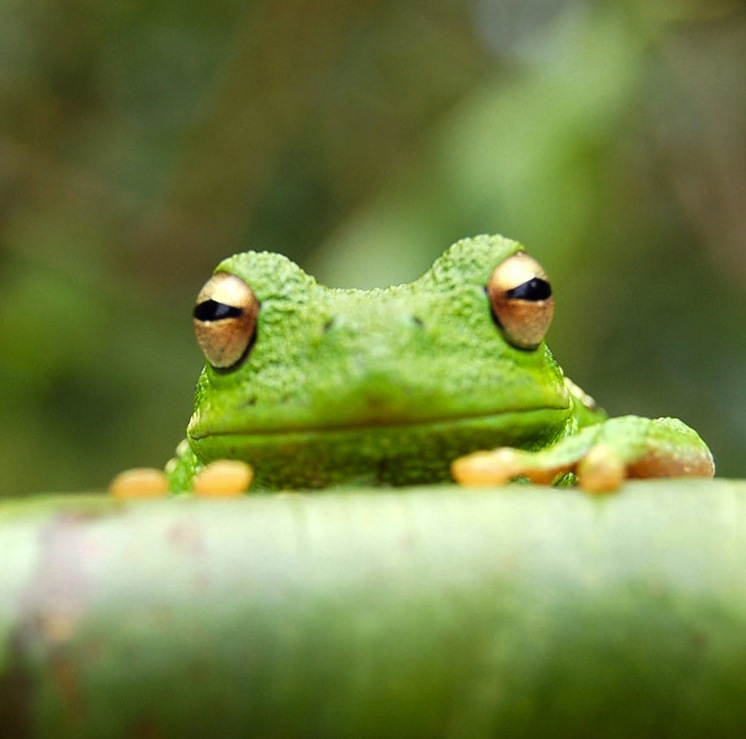
\includegraphics[width=\hsize]{frog}
\caption{A half-columnwidth image using wrapfigure, to be used sparingly. Note that using a wrapfigure before a sectional heading, near other floats or page boundaries is not recommended, as it may cause interesting layout issues. Use the optional argument to wrapfigure to control how many lines of text should be set half-width alongside it.}
\label{fig:halfwidth}
\end{wrapfigure}

Some filler text to sit alongside the half-width figure. \lipsum[1-2]

\begin{figure}
\begin{fullwidth}
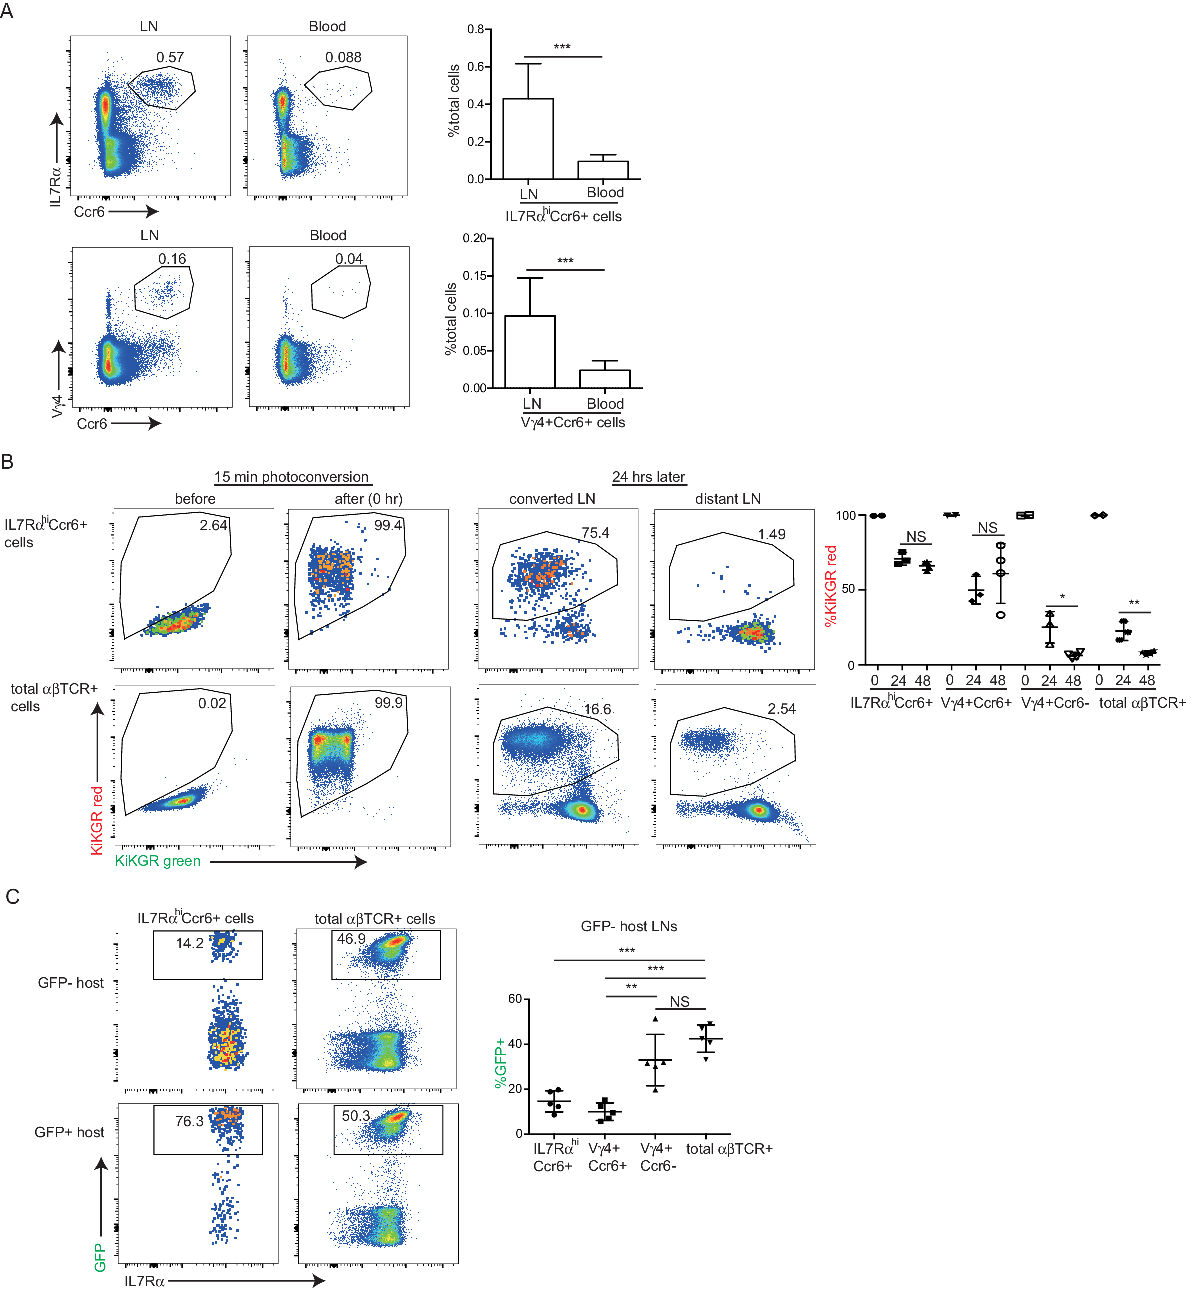
\includegraphics[width=0.95\linewidth]{elife-18156-fig2}
\caption{A very wide figure that takes up the entire page, including the gutter space.}
\label{fig:fullwidth}
\figsupp{There is no limit on the number of Figure Supplements for any one primary figure. Each figure supplement should be clearly labelled, Figure 1--Figure Supplement 1, Figure 1--Figure Supplement 2, Figure 2--Figure Supplement 1 and so on, and have a short title (and optional legend). Figure Supplements should be referred to in the legend of the associated primary figure, and should also be listed at the end of the article text file.}{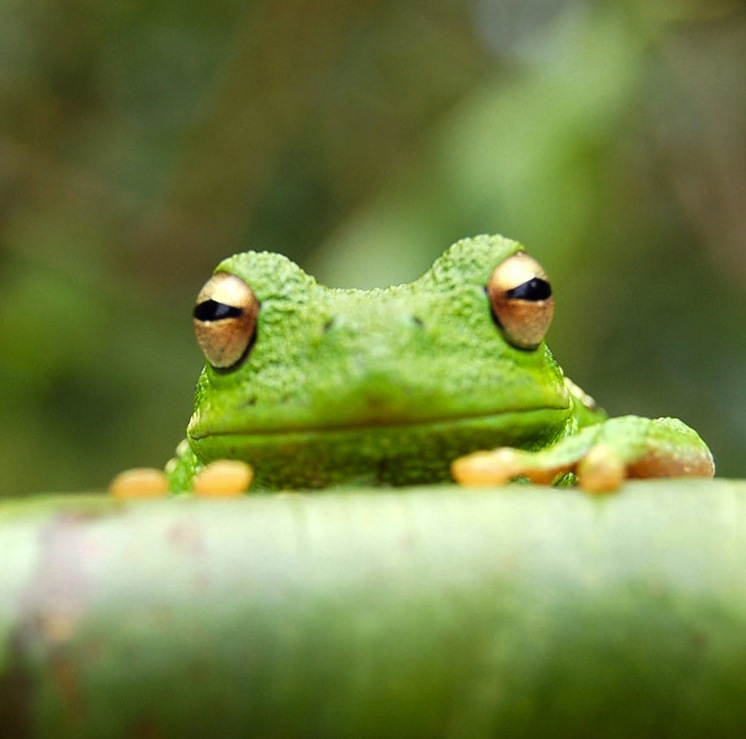
\includegraphics[width=6cm]{frog}}
\end{fullwidth}
\end{figure}

\subsection{Citations}

LaTeX formats citations and references automatically using the bibliography records in your .bib file, which you can edit via the project menu. Use the \verb|\cite| command for an inline citation, like \cite{Aivazian917}, and the \verb|\citep| command for a citation in parentheses \citep{Aivazian917}. The LaTeX template uses a slightly-modified Vancouver bibliography style. 

\begin{featurebox}
\caption{This is an example feature box}
\label{box:simple}
This is a feature box. It floats!
\medskip

\includegraphics[width=5cm]{example-image}
\featurefig{`Figure' and `table' captions in feature boxes should be entered with \texttt{\textbackslash featurefig} and \texttt{\textbackslash featuretable}. They're not really floats.}

\lipsum[1]
\end{featurebox}

\subsection{Mathematics}

\LaTeX{} is great at typesetting mathematics. Let $X_1, X_2, \ldots, X_n$ be a sequence of independent and identically distributed random variables with $\text{E}[X_i] = \mu$ and $\text{Var}[X_i] = \sigma^2 < \infty$, and let
\begin{equation}
\label{eq:CLT}
S_n = \frac{X_1 + X_2 + \cdots + X_n}{n}
      = \frac{1}{n}\sum_{i}^{n} X_i
\end{equation}
denote their mean. Then as $n$ approaches infinity, the random variables $\sqrt{n}(S_n - \mu)$ converge in distribution to a normal $\mathcal{N}(0, \sigma^2)$.

\lipsum[3]

\begin{figure}
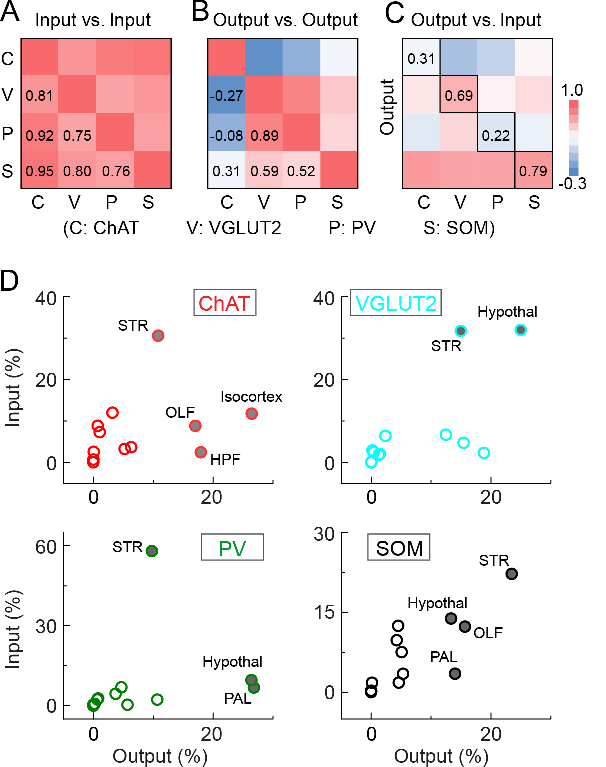
\includegraphics[width=\linewidth]{elife-13214-fig7}
\caption{A text-width example.}
\label{fig:view}
%% If the optional argument in the square brackets is ``none'', then the caption *will not appear in the main figure at all* and only the full caption will appear under the supplementary figure at the end of the manuscript.
\figsupp[Shorter caption for main text.]{This is a supplementary figure's full caption, which will be used at the end of the manuscript.}{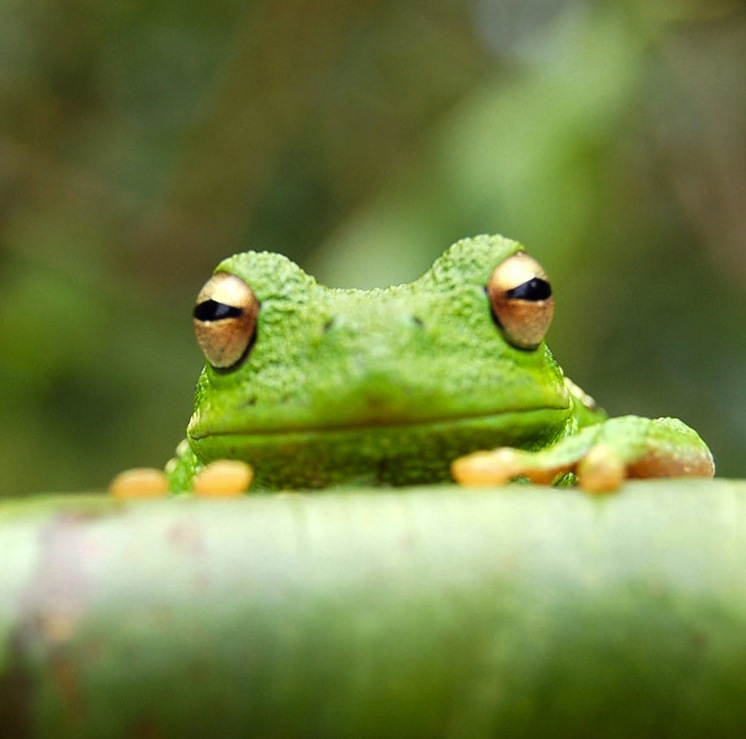
\includegraphics[width=6cm]{frog}}
\figsupp{This is another supplementary figure.}{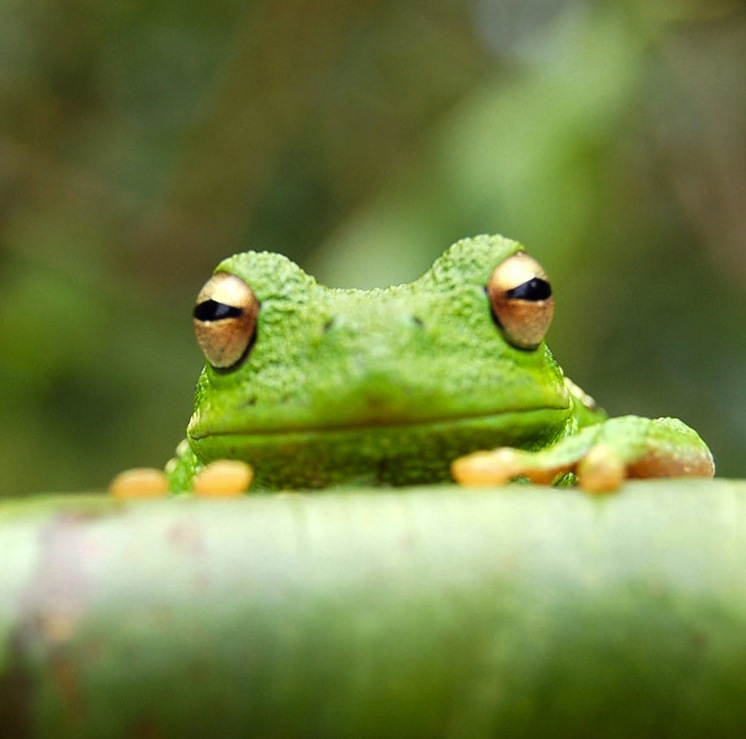
\includegraphics[width=6cm]{frog}}
\figdata{This is a description of a data source.}
\figdata{This is another description of a data source.}
\end{figure}

\subsection{Other Chemistry Niceties}

You can use commands from the \texttt{mhchem} and \texttt{siunitx} packages. For example: \ce{C32H64NO7S}; \SI{5}{\micro\metre}; \SI{30}{\degreeCelsius}; \SI{5e-17}{\Molar}

\subsection{Lists}

You can make lists with automatic numbering \dots

\begin{enumerate}
\item Like this,
\item and like this.
\end{enumerate}
\dots or bullet points \dots
\begin{itemize} 
\item Like this,
\item and like this.
\end{itemize}
\dots or with words and descriptions \dots
\begin{description}
\item[Word] Definition
\item[Concept] Explanation
\item[Idea] Text
\end{description}

Some filler text, because empty templates look really poorly. \lipsum[1]


\section{Acknowledgments}

Funder and other information can be given here.

\nocite{*} % This command displays all refs in the bib file
\bibliography{transport_properties}

%%%%%%%%%%%%%%%%%%%%%%%%%%%%%%%%%%%%%%%%%%%%%%%%%%%%%%%%%%%%
%%% APPENDICES
%%%%%%%%%%%%%%%%%%%%%%%%%%%%%%%%%%%%%%%%%%%%%%%%%%%%%%%%%%%%

\appendix
\begin{appendixbox}
\label{first:app}
\section{Firstly}
\lipsum[1]

%% Sadly, we can't use floats in the appendix boxes. So they don't ``float'', but use \captionof{figure}{...} and \captionof{table}{...} to get them properly caption.
\begin{center}
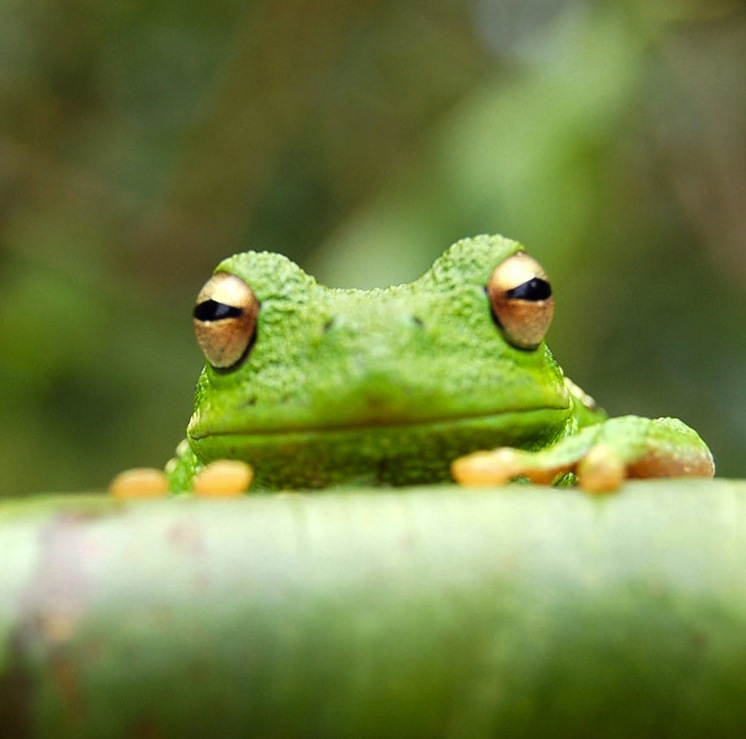
\includegraphics[width=\linewidth,height=7cm]{frog}
\captionof{figure}{This is a figure in the appendix}
\end{center}

\section{Secondly}

\lipsum[5-8]

\begin{center}
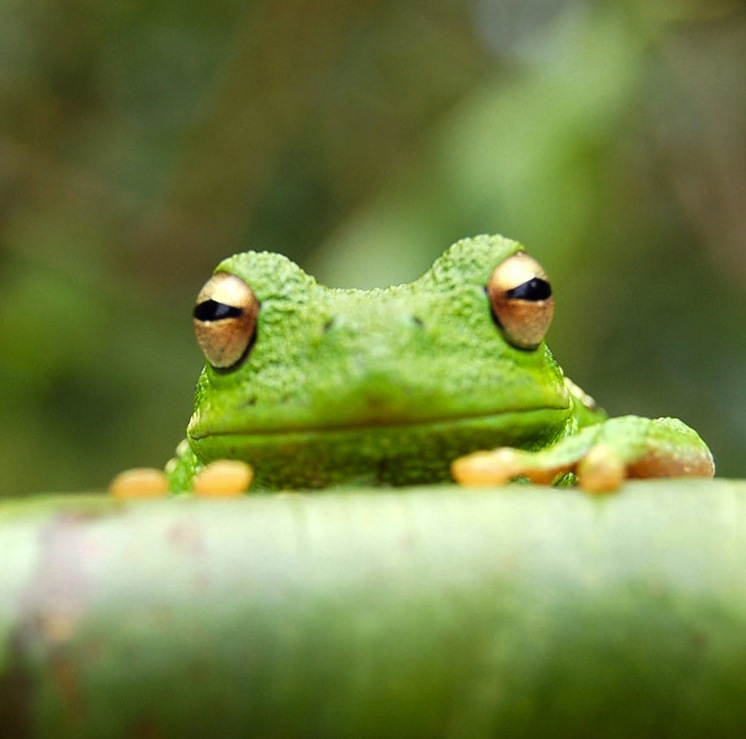
\includegraphics[width=\linewidth,height=7cm]{frog}
\captionof{figure}{This is a figure in the appendix}
\end{center}

\end{appendixbox}

\begin{appendixbox}
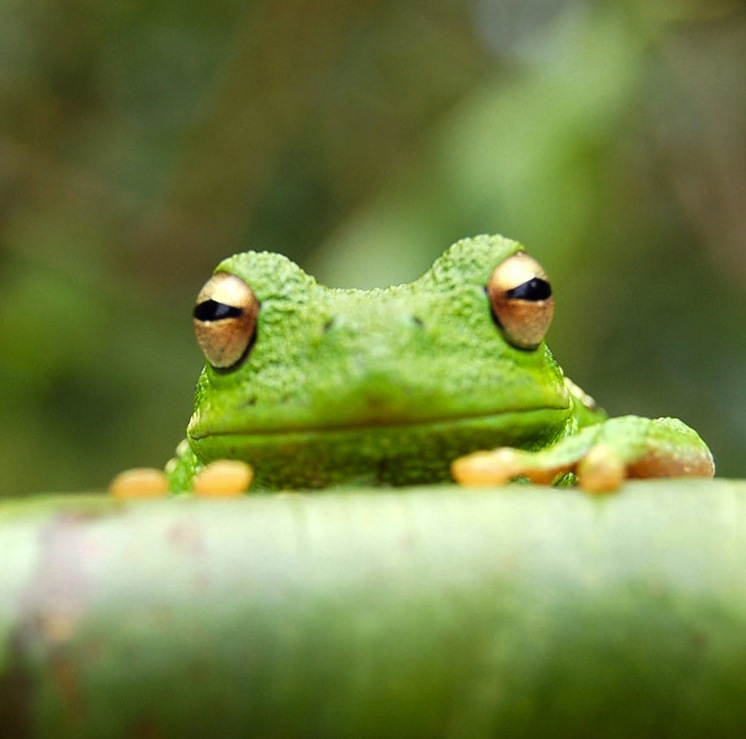
\includegraphics[width=\linewidth,height=7cm]{frog}
\captionof{figure}{This is a figure in the appendix}
\end{appendixbox}
\end{document}